\chapter{Data and Methodology}
\label{chap:data_methodology}

This section details the data sources and methodological approaches employed in this thesis. It begins by describing the primary data source, the ICIJ Offshore Leaks Database (Section \ref{sec:3_1}), and the external datasets used for constructing the primary features (Section \ref{sec:3_2}). Subsequently, it introduces a novel methodology utilizing agentic AI to enrich a sample of the intermediaries from the ICIJ dataset, classifying them into the typology of De Groen (2017) based on their online presence (Section \ref{sec:3_3}). Finally, there is an outline of the general quantitative techniques applied (Section \ref{sec:3_4}).

\section{The ICIJ Offshore Leaks Database}
\label{sec:3_1}

The primary empirical basis for this thesis is the International Consortium of Investigative Journalists (ICIJ) Offshore Leaks Database. 

\subsection{Overview}

Our primary dataset is the International Consortium of Investigative Journalists (ICIJ) Offshore Leaks Database (ICIJ, n.d.). This publicly accessible repository is a collation of a series of leaks, most notably the Offshore Leaks (2013), Panama Papers (2016), Paradise Papers (2017/18), and Pandora Papers (2021/22). The database is substantial, cataloging information on over 810,000 offshore entities encompassing a range of structures such as companies, trusts, and foundations, and establishing connections to more than 750,000 individuals and corporate entities. These connections span over 200 countries and territories, with the underlying records covering a significant historical period, in some cases extending up to the year 2020. Figure \ref{fig:incorporations_time} is an overview of when the entities included in the dataset were incorporated.

\begin{figure}[htbp]
    \centering
    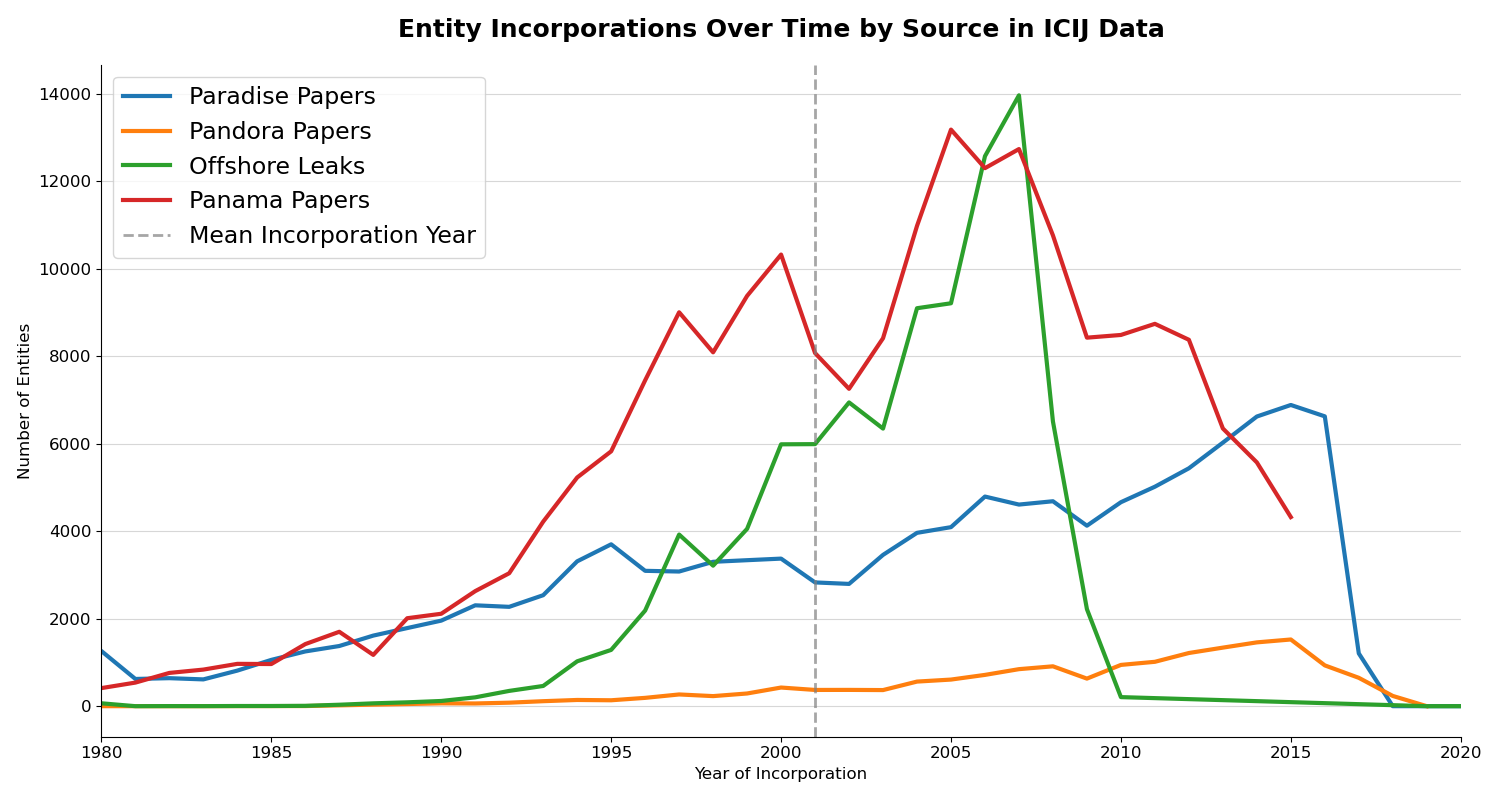
\includegraphics[width=0.8\textwidth]{Preliminary_Incorporations_over_Time.png}
    \caption{Overview of Entity Incorporations Over Time in ICIJ Data}
    \label{fig:incorporations_time}
\end{figure}

The fundamental data model leveraged by the ICIJ data is a graph. This model is used for its ability to represent interconnected information, conceptualizing data as \textbf{nodes} (the core informational units) and \textbf{edges} (the links defining how these units are connected). For the purposes of our study, the most pertinent node types are:

\begin{itemize}
    \item \textbf{Entities}: These represent the diverse offshore legal structures documented in the leaks, such as Limited companies, S.A. (Société Anonyme), Inc. (Incorporated), trusts, and foundations.
    \item \textbf{Officers}: This category includes individuals or, in some instances, other corporate bodies that fulfill specific roles (e.g., director, shareholder, beneficial owner, trustee, protector, nominee) attachted to an Entity.
    \item \textbf{Intermediaries}: These are the professional facilitators - typically law firms, accounting practices, banks, trust companies, or specialized middlemen - who assist clients in the establishment and ongoing management of offshore entities. They often act as the liaison with offshore service providers like Mossack Fonseca or Appleby that provide the underlying incorporation service.
\end{itemize}

Relationships (edges) within this graph structure explicitly define the nature of the connections, for example, an Officer is an \texttt{officer\_of} an Entity, or an Intermediary acts as an \texttt{intermediary\_of} an Entity.

The two primary node types of interest for this thesis are \textbf{Entities} and, critically, \textbf{Intermediaries}. In the ICIJ data model, the role of intermediaries is, with very few exceptions, represented entirely through their connections to Entities. That is, at a high level, the relational pathway is: Intermediaries are \texttt{intermediary\_of} Entities, which in turn have Officers (who are \texttt{officer\_of} these Entities).

Figure \ref{fig:sample_network} is a simplified illustration of how one sample sub-network of the ICIJ data model could look. Officers are connected to entities, that have been incorporated by intermediaries with the help of a service provider. The ICIJ dataset can, at a high level, be viewed as a collection of such sub-networks. 

\begin{figure}[htbp]
    \centering
    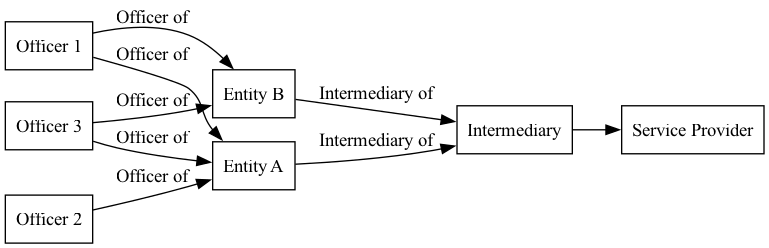
\includegraphics[width=0.8\textwidth]{Methods_Sample_Network.png}
    \caption{Overview of how Intermediaries appear in ICIJ Data Model}
    \label{fig:sample_network}
\end{figure}

The following subsections will go more in detail with each of the node types.

\subsection{Entities}

At the entity level, key data points include the entity's registered \texttt{name}, its \texttt{jurisdiction} of incorporation (which is standardized to ISO3 country codes for consistent geographical analysis), and the \texttt{country\_codes} associated with its operational activities or linked addresses. These \texttt{country\_codes} are often distinct from its legal \texttt{jurisdiction} of incorporation and provide information on the geographical location of the entity's actual business or connections. Additionally, we have the entity's \texttt{incorporation\_date}, its operational \texttt{status} (e.g., Active, Struck Off, Dissolved), and its specific \texttt{entity\_type} (e.g., Standard International Company, Trust, Business Company Limited by Shares).

A feature we construct at the entity-level is the \texttt{bearer\_count}. This metric quantifies the number of associated officers explicitly identified as "Bearer" or its equivalents (e.g., "THE BEARER," "EL PORTADOR"). The presence of bearer instruments, as highlighted by Harrington (2016), is a critical indicator of mechanisms used to obscure true beneficial ownership. In such arrangements, legal ownership follows the physical possession of the share certificate rather than being recorded in a central register, thereby enhancing anonymity (Chang et al., 2023b).

\subsection{Intermediaries and Feature Engineering}

For \textbf{intermediaries}, the analysis extends beyond basic identifying information. Beyond their \texttt{name} and the \texttt{countries} associated with their operational addresses, we calculate their \texttt{degree}. In this context, the degree represents the total number of distinct entities an intermediary is connected to within the ICIJ network, serving as a proxy for their client base size and activity level.

More extensively, we construct several aggregated metrics that characterize each intermediary based on the collective properties of the entities they service. As our primary research interest lies in understanding the roles and specializations of intermediaries, we aggregate information at the intermediary-level about the entities they are connected to. While graph data models excel at representing complex, interrelated data, tabular data is a lot easier to work with. By this manner, sub-graphs composed of entities and intermediaries are summarised into tabular features, aggregating the most important information about the entities they service. This way, rather than having to work with the full graph structure, we can work with a table of intermediaries, each summarised by their connections to entities. 

For every intermediary, we generate the following features:

\begin{itemize}
   \item \texttt{country\_counts}: A dictionary detailing the frequency of entities they are connected to, grouped by the \texttt{country\_codes} associated with those entities. This reflects the geographical spread of the operational links of the entities they service. A concrete example would be an intermediary connected to 10 entities in the United States and 5 in the United Kingdom, resulting in this intermediary having a \texttt{country\_counts} of \{ "USA": 10, "GBR": 5\}. 
   \item \texttt{jurisdiction\_counts}: A dictionary detailing the frequency of entities they are connected to, grouped by the \texttt{jurisdiction} (ISO3 code) in which those entities are incorporated. This captures the intermediary's usage of different offshore legal environments.
   \item \texttt{regime\_counts}: A dictionary detailing the frequency of entities they are connected to, grouped by the political regime type (e.g., Liberal Democracy, Closed Autocracy, as per V-Dem data detailed in Section \ref{sec:3_2}) of the entities' associated \texttt{country\_codes} at the time of entity incorporation. This provides insight into the political contexts linked to an intermediary's client base. 
   \item \texttt{legal\_tech\_counts}: A dictionary detailing the frequency of entities they are connected to, grouped by the predominant types of "legal technologies" (e.g., Banking, Corporate, Dual-Purpose, as per Laffitte (2024), detailed in Section \ref{sec:3_2}) prevalent in the entities' jurisdictions of incorporation at the time of their formation. This reflects an intermediary's engagement with specific offshore legal architectures.
   \item \texttt{bearer\_share}: Lastly, we quantify for each intermediary the number of entities they are connected to that have \texttt{bearers\_connected} (i.e., entities with a \texttt{bearer\_count} > 0 - recall that this was based on the officers they were connected to) and calculate the \texttt{bearer\_share}, representing the proportion of their serviced entities that utilize these anonymity-enhancing instruments.
\end{itemize}

To measure the diversity of their client entity portfolio across these dimensions, we also compute normalized entropy scores: \texttt{country\_entropy}, \texttt{jurisdiction\_entropy}, \texttt{regime\_entropy}, and \texttt{legal\_tech\_entropy}. More on that specific measure in Section \ref{subsec:entropy}. The important part to take away at this stage is, that these scores provide a measure of the diversity of the intermediary's client base across the respective dimensions, with higher values indicating a more diverse portfolio. For example, a high jurisdiction-entropy means an intermediary uses a lot of jurisdictions relative to the number of entities they have incorporated.

\section{Other Data Sources}
\label{sec:3_2}
To enrich the core ICIJ data, several external datasets are integrated, primarily to provide contextual information at the country or jurisdiction level, and to classify intermediaries by type.

Going into more detail with the external datasets:

\begin{enumerate}
    \item The \textbf{Varieties of Democracy (V-Dem) Project data}: We utilize the \texttt{v2x\_regime} variable from VDem's comprehensive dataset to enrich our entity data. This variable classifies countries into categories such as Closed Autocracy, Electoral Autocracy, Electoral Democracy, or Liberal Democracy. Its methodology relies on a sufficient number of experts to classify it, which are not available in Micro-states. Therefore, empty fields in V-Dem are imputed as "Microstate" though its not quite conceptually similar to the other categories, but a fitting descriptive label nonetheless. By matching an entity's associated \texttt{country\_codes} (representing operational links) and its \texttt{incorporation\_year} with the VDem data for the corresponding country and year, we assign a political regime classification to each entity. The idea is, regimes capture very concisely a lot of information about which context a client has and is established in e.g. Chang et al. (2023b). This entity-level regime information is then aggregated to construct the \texttt{regime\_counts} at the intermediary level, providing insight into the political environments linked to an intermediary's clientele.
  
  \item \textbf{Laffitte's (2024) "The Market for Tax Havens" dataset} (specifically \texttt{HTHD.csv}): This dataset offers a historical perspective on the "offshore legal architecture" of various jurisdictions, detailing their adoption of different "legal technologies" such as International Business Company (IBC) laws, trust legislation, or banking secrecy provisions. Laffitte categorizes these into broader types such as "Banking," "Corporate," "Dual-Purpose" (e.g., IBCs serving both personal and corporate needs), and "Personal" (e.g., trust laws). We merge this dataset onto our entity data by matching the entity's \texttt{jurisdiction} of incorporation and its \texttt{incorporation\_year} with the HTHD data. This allows us to identify the specific legal technologies active in an entity's jurisdiction at its time of incorporation. This entity-level characterization is subsequently aggregated to create the \texttt{legal\_tech\_counts} at the intermediary level, reflecting the types of legal environments their serviced entities operate within.
\end{enumerate}

\section{Agentic AI for Intermediary Classification}
\label{sec:3_3}

Directly at the Intermediaries-level, we also enrich a random \textbf{subset of intermediaries} and another subset of the most connected intermediaries with information on their specific "type." This classification is based on the typology adapted from the De Groen (2017) and covered in the theory section. 

The core idea is to use an AI agent loop to automate the process of gathering the information about intermediaries that's online, whether it be incorporation documents or their own online presence (e.g. a lot of them have some kind of LinkedIn profile). After three iterative searches, an LLM (gemini-2.0-flash) determines whether there is sufficent information to classify them, and if so, categorises them into the four-fold typology, providing a reasoning. The basic workflow is illustrated in Figure \ref{fig:agent_loop_placeholder}. More detail on the agentic AI methodology is provided appendix and the code on GitHub along with the rest of the replication code.

\begin{figure}[htbp]
    \centering
    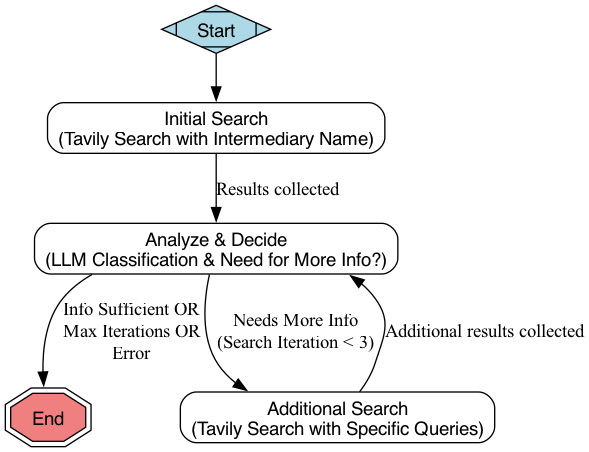
\includegraphics[width=0.8\textwidth]{Methods_Agent_Graph.png}
    \caption{Agent Setup for Intermediary Classification}
    \label{fig:agent_loop_placeholder}
\end{figure}

\section{Analytical and Statistical Techniques}
\label{sec:3_4}

This section outlines the core analytical techniques applied to the processed data. At a high-level, they are 1) a measure of concentration/diversity, choosing entropy as the preferred one, 2) an approach to adjust significance thresholds, choosing the conservative Bonferroni method, given the exploratory nature of the analysis, and 3) a range of different statistical tests - mostly non-paremetric - to assess the significance of the results.

\subsection{Entropy}
\label{subsec:entropy}
Drawing on its application in prior studies of offshore finance (e.g., Chang et al., 2023b; Kejriwal \& Dang, 2020), Shannon entropy is employed as a measure of diversity or concentration. For a discrete random variable $X$ with $n$ possible outcomes $x_1, ..., x_n$ and probabilities $p(x_i)$, entropy is defined as:
\begin{equation}
    H(X) = -\sum_{i=1}^{n} p(x_i) \log_b p(x_i)
\end{equation}
where $b$ is the base of the logarithm (typically $b=2$, yielding units of bits). Compared to other concentration measures like the Herfindahl-Hirschman Index (HHI), entropy gives more weight to smaller amounts of diversity. This characteristic is particularly useful in this thesis, as intermediaries' activities (e.g., choice of jurisdictions or countries) are often highly concentrated in one or two locations, so entropy yields greater variation and thereby more statistical power compared to other common concentration measures like HHI. Normalized entropy, calculated by dividing $H(X)$ by the maximum possible entropy ($\log_b n$), is used to provide a standardized measure (0 to 1) for comparing diversity across intermediaries with different breadths of activity. Entropy is used, for example, as a summary statistic at the intermediary-level to quantify the diversity of their client entity portfolio across dimensions like country, jurisdiction, or regime type, enabling subsequent comparisons of these distributions across different intermediary classifications.

\subsection{Multiple Hypothesis Testing}
\label{subsec:multiple_hypothesis_testing}
Given that this thesis is highly exploratory and investigates a multitude of potential associations, it is important to address the issue of multiple hypothesis testing. When numerous statistical tests are performed, the Type I error rate (choosing here, as conventional, 5\%) does not hold. To counteract this, a highly conservative approach is adopted, opting for the \textbf{Bonferroni correction} to control the Family-Wise Error Rate (FWER) at the conventional maximum of 5\%. This method adjusts the significance threshold for each individual test to $\alpha/m$, where $\alpha$ is the desired FWER (e.g., 0.05) and $m$ is the total number of hypotheses tested. Concretely, if we test 100 hypotheses assuming no true effects, in expectation, we would expect 5 of them to be false positives at the conventional 5\% significance level. To control for this, the Bonferroni correction would set the significance threshold for each individual test to $0.05/100 = 0.0005$ hereby ensuring that the overall probability of making at least one Type I error across all tests remains at or below 5\%.

\subsection{Significance Tests}
\label{subsec:significance_testing}

The above covers our adjustments of when we consider a test significant; this subsection proceeds to cover the specific statistical tests we use to assess the significance of the results we observe. These tests are chosen for their robustness to violations of normality assumptions, which is critical given the nature of our data which often exhibits characteristics such as power-law distributions and involves categorical or count-based measures derived from network structures and financial activities where we cannot expect the Central Limit Theorem and the usual asymptotics to hold because of, for instance, the potentially non-finite moments of the distribution (Hastie et al. 2009; Kejriwal \& Dang, 2020; Alstadsæter et al., 2019). The following methods are applied in the empirical analysis chapter. Zar (2010) is the main reference point for the statistical tests employed.
\begin{itemize}
    \item \textbf{Mann-Whitney U test}: A non-parametric test used for comparing the central moments between two independent groups. It is particularly useful when the data is not normally distributed, as is often the case with metrics like entropy scores or network-derived measures. For this thesis, this is crucial for comparing, for example, the distribution of network centrality scores or jurisdiction diversity measures (e.g., entropy scores) between different classifications of intermediaries (e.g., 'Legal Expert' vs. 'Administrator'), where underlying normality cannot be assumed.

    \item \textbf{Fisher's exact test}: Employed for analyzing categorical data, particularly in contingency tables (e.g., 2x2 tables). This test is ideal for assessing associations between categorical variables, such as those resulting from association analysis or when examining the relationship between dummy variables (e.g., whether entities are connected to bearer instruments and intermediary type). It is an exact test, making it suitable for small sample sizes or when expected cell counts are low. Given that our dataset involves numerous categorical attributes-such as the classification of intermediaries, the jurisdiction of entity incorporation, or the use of specific secrecy tools like bearer shares - Fisher's exact test is indispensable.

    \item \textbf{Two-sample Kolmogorov-Smirnov test}: Used for comparing the underlying distributions of continuous variables from two independent samples. Unlike tests that compare central tendencies (like the t-test or Mann-Whitney U), the K-S test is sensitive to differences in location, scale, and shape of the distributions, offering a more comprehensive comparison. This test is particularly useful when we are interested in whether two groups of entities or intermediaries differ not just in their central tendencies but in the overall shape, spread, or skewness of their associated metrics and distribution. For example, the K-S test is used to compare the entire degree distribution of intermediaries specializing in 'Tax Expert' services versus those classified as 'Investment Advisors', providing more power and sensitivity beyond what a simple comparison of medians or means might offer. This is especially relevant for network-derived measures which, as discussed, often follow non-normal, potentially power-law, distributions (Kejriwal \& Dang, 2020; Chang et al., 2023a).
\end{itemize}


